\documentclass[11pt]{article}
\usepackage{amsmath,amssymb,amsthm}
\usepackage{booktabs}
\usepackage{tikz}
\newtheorem{theorem}{Theorem}[section]
\newtheorem{lemma}[theorem]{Lemma}
\theoremstyle{definition}
\newtheorem{definition}[theorem]{Definition}

\title{A Reflow Lab Smoke Test}
\author{The Reflow Lab}
\date{}

\begin{document}
\maketitle

\begin{abstract}
  This two-page article exercises the pieces a real paper brings to the
  reflow derivation: sectioning, theorem environments, a list, aligned
  display mathematics, a footnote, a small table, a picture, and a
  citation resolved through \textsc{Bib}\TeX. It exists so that the
  harness in \texttt{scripts/reflow-lab} has something to test itself on
  before any corpus paper is added.
\end{abstract}

\section{Introduction}

Every reflowed paper starts as a node list. The serializer records what
\LaTeX{} typeset, paragraph by paragraph, and the encode step turns the
record into blocks a browser can lay out again at any width~\cite{knuth84}.
The oracle then compares the glyph text of that stream with the text layer
of the printed PDF\footnote{The comparison tolerates hyphenation, ligatures,
and running heads, but not a dropped section.} and refuses to seal a bundle
that reads differently from the paper beside it.

The smoke test checks three things in particular:
\begin{itemize}
  \item that display mathematics survives as a display and not as a
    run-in formula,
  \item that a footnote's text is carried once rather than twice, and
  \item that the picture below arrives as vector graphics with its
    labels in place.
\end{itemize}

\section{A theorem and its proof}

\begin{definition}
  A natural number $p > 1$ is \emph{prime} if its only positive divisors
  are $1$ and $p$.
\end{definition}

\begin{theorem}[Euclid]\label{thm:euclid}
  There are infinitely many primes.
\end{theorem}

\begin{proof}
  Suppose $p_1, \dots, p_n$ were all the primes and consider
  $N = p_1 p_2 \cdots p_n + 1$. No $p_i$ divides $N$, since each leaves
  remainder $1$; so a prime factor of $N$ lies outside the list, which is
  absurd~\cite{euclid}.
\end{proof}

Two identities the reader may check on a napkin:
\begin{align}
  \sum_{k=1}^{n} k &= \frac{n(n+1)}{2}, \label{eq:gauss} \\
  \sum_{k=1}^{n} k^3 &= \left( \frac{n(n+1)}{2} \right)^{2} .
\end{align}
Equation~\eqref{eq:gauss} is the one every schoolchild is told Gauss found;
the second says the cubes sum to the square of the first.

\begin{lemma}
  For every real $x$, $\lfloor x \rfloor \le x < \lfloor x \rfloor + 1$.
\end{lemma}

\section{A table and a picture}

Table~\ref{tab:sizes} lists a few small numbers. They are chosen so that no
row of the table is a page number in disguise: the oracle strips a line
that holds nothing but an integer, and a table of bare integers would be
the wrong place to find out.

\begin{table}[ht]
  \centering
  \begin{tabular}{lrr}
    \toprule
    Object & Count & Weight (kg) \\
    \midrule
    Pebbles & 12 & 0.4 \\
    Bricks & 3 & 6.9 \\
    Anvils & 1 & 55.0 \\
    \bottomrule
  \end{tabular}
  \caption{Three objects, by count and weight.}
  \label{tab:sizes}
\end{table}

Figure~\ref{fig:path} is a picture: a directed path with a highlighted
vertex and a partially transparent region behind it, which is exactly the
kind of drawing the in-image converter used to flatten.

\begin{figure}[ht]
  \centering
  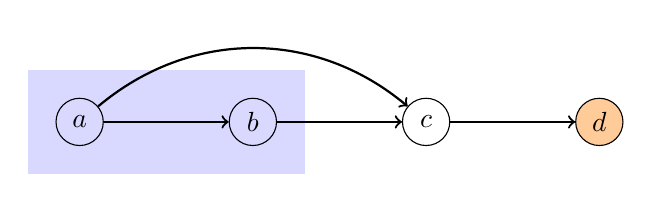
\begin{tikzpicture}[scale=1.1, every node/.style={draw, circle, minimum size=6mm, inner sep=1pt}]
    \fill[blue, opacity=0.15] (-0.6,-0.6) rectangle (2.6,0.6);
    \node (a) at (0,0) {$a$};
    \node (b) at (2,0) {$b$};
    \node (c) at (4,0) {$c$};
    \node[fill=orange!40] (d) at (6,0) {$d$};
    \draw[->, thick] (a) -- (b);
    \draw[->, thick] (b) -- (c);
    \draw[->, thick] (c) -- (d);
    \draw[->, thick, bend left=40] (a) to (c);
  \end{tikzpicture}
  \caption{A directed path on four vertices, with a shortcut.}
  \label{fig:path}
\end{figure}

\section{Some prose to reach the second page}

A reflowed view is only useful if it reads like the paper. Long paragraphs
are where line breaking, hyphenation, and inter-word spacing are decided,
so this section carries enough of them to push the document onto a second
page and to give the narrow rendering something to reflow. None of the
sentences here say anything the earlier sections did not; they are ballast,
and ballast is exactly what a smoke test needs.

The first paragraph of ballast talks about widths. At eleven hundred pixels
the column is wide and the lines are long; at seven hundred the column is
narrow and the same paragraph breaks into nearly twice as many lines. The
harness records both, and the report shows the narrow rendering only for
the first two slices, since the shape of the break is visible at the top.

The second paragraph of ballast talks about fonts. The text face is
Computer Modern on the printed side and Latin Modern on the web side, the
mathematics is set from the legacy Type~1 outlines in both, and every glyph
the viewer cannot find is marked so the harness can count it. A count above
zero is a bug in the export or the font map, never in the paper.

The third paragraph of ballast talks about pictures. The picture above was
externalized by \texttt{tikz}, converted inside the pinned \TeX{} image, and
sanitized by the encode step. Its transparent rectangle is the test: a
converter that flattens transparency turns the whole drawing into a raster,
and the sanitizer then drops the raster, so the figure would arrive empty.

The fourth and last paragraph of ballast talks about the bibliography that
follows. It is generated by \textsc{Bib}\TeX{} from a two-entry file, which
means \texttt{latexmk} must run the bibliography tool during the compile,
and the reflowed view must carry the reference list exactly as printed.

\bibliographystyle{plain}
\bibliography{refs}

\end{document}
